%%% for presentation mode
\documentclass[14pt]{beamer}

%%% for article mode
%\documentclass[14pt]{article}
%\usepackage{beamerarticle}
%\usepackage[unicode]{hyperref}

\usepackage{CJKutf8}
\usepackage{graphicx}
\usepackage{xcolor}
%\DeclareGraphicsExtensions{.bb,.pdf,.jpg,.png,.tif}
%\pdfimageresolution 100
%\usepackage{color}

%% handout
%\usepackage{pgfpages}
%\pgfpagesuselayout{4 on 1}[a4paper,border shrink=5mm,landscape]

%\hypersetup{bookmarks=true,pdfauthor=letoh,colorlinks=true,linkcolor=black,pdfpagemode=FullScreen}
\hypersetup{pdfauthor=letoh,colorlinks=true,linkcolor=magenta,pdfpagemode=FullScreen}
%\hypersetup{pdfauthor=letoh,colorlinks=true,linkcolor=black,pdfpagemode=FullScreen}

\usepackage{listings}
\lstset{tabsize=4,language=Python,
	%frameround=ffft,
	%frame=shadowbox,
	showstringspaces=false,
	basicstyle=\footnotesize\ttfamily,
	keywordstyle=\color{blue}\bfseries,
	stringstyle=\color{red},
	commentstyle=\color{OliveGreen}\ttfamily\itshape}

\mode<presentation>
{
	\usetheme{PyHug}
	%\usetheme{Warsaw}
%  \setbeamercovered{transparent}
  % or whatever (possibly just delete it)
  \setbeamercovered{dynamic}
%  \setbeamercovered{invisible}
}



\newcommand{\alertframe}[1]{
	\begin{frame}
		\begin{center}
			\alert{\textbf{\Huge #1}}
		\end{center}
	\end{frame}
}

\newcommand{\popupframe}[1]{
	\begin{frame}
		\begin{center}
			\textbf{\Huge #1}
		\end{center}
	\end{frame}
}

%\usepackage{times}
%\usepackage[latin1]{inputenc}

\title{Depana: A Toy Static Dependency Analyzer}
\author{letoh}
\institute{PyHug::January}
%\date{\today}
\date{January 9, 2012}

\begin{document}
\begin{CJK}{UTF8}{nsung}
% View this in acroread with "loop after last page option" in full screen mode.


%\AtBeginSubsection[]
%{
%	\begin{frame}<presentation>
%		\frametitle{Outline}
%		\tableofcontents[currentsection,currentsubsection]
%	\end{frame}
%}


%
% Title
%
\begin{frame}
  \titlepage
\end{frame}


%
% Outline
%
\section*{Outline} 
%\frame{\tableofcontents}
\begin{frame}
  \frametitle{Outline}
  \tableofcontents
  % You might wish to add the option [pausesections]
\end{frame}


% vim: enc=utf8:tenc=big5

%%%%%%%%%%%%%%%%%%%%%%%%%%%%%%%%%%%%%%%%%%%%%%%%%%%%%%%%%%%%%%%%%%%%%%%%%%%%%%
%%%%%%%%%%%%%%%%%%%%%%%%%%%%%%%%%%%%%%%%%%%%%%%%%%%%%%%%%%%%%%%%%%%%%%%%%%%%%%
%%%%%%%%%%%%%%%%%%%%%%%%%%%%%%%%%%%%%%%%%%%%%%%%%%%%%%%%%%%%%%%%%%%%%%%%%%%%%%
\section{Static Analysis}
\begin{frame}[t]
	\frametitle{Purpose}
	\begin{itemize}
		\item<+-|alert@+> to understand software architecture
		\begin{itemize}
			\item<+-|alert@+> organization
			\item<+-|alert@+> relationship
			\item<+-|alert@+> execution flow
		\end{itemize}
		\item<+-|alert@+> to find the defects in the program
		\begin{itemize}
			\item<+-|alert@+> memory leak
			\item<+-|alert@+> dangling pointer
		\end{itemize}
	\end{itemize}
\end{frame}



%%%%%%%%%%%%%%%%%%%%%%%%%%%%%%%%%%%%%%%%%%%%%%%%%%%%%%%%%%%%%%%%%%%%%%%%%%%%%%
%%%%%%%%%%%%%%%%%%%%%%%%%%%%%%%%%%%%%%%%%%%%%%%%%%%%%%%%%%%%%%%%%%%%%%%%%%%%%%
%%%%%%%%%%%%%%%%%%%%%%%%%%%%%%%%%%%%%%%%%%%%%%%%%%%%%%%%%%%%%%%%%%%%%%%%%%%%%%
\section{Dependency}
\popupframe{What is Dependency?}

\begin{frame}[plain]
	\begin{center}
		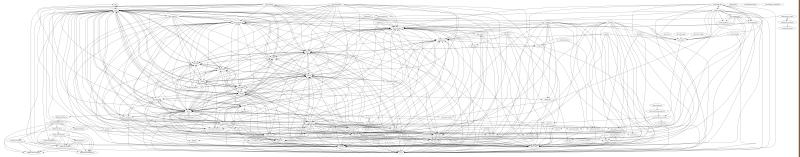
\includegraphics[scale=0.4]{gcin-2-6-5.png}
	\end{center}
\end{frame}

\alertframe{W○F!}

\begin{frame}[plain]
	\begin{center}
		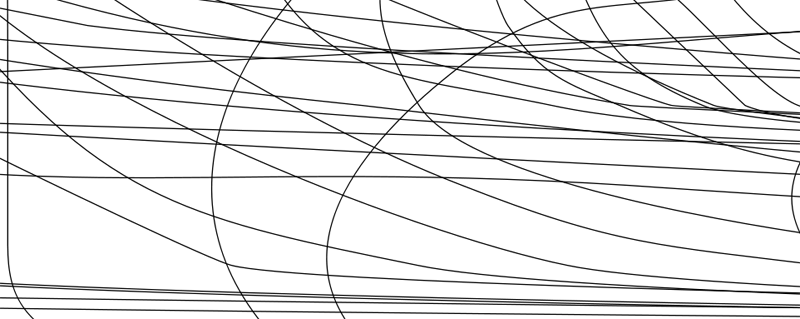
\includegraphics[scale=0.4]{gcin-2-6-5-2.png}
	\end{center}
\end{frame}

\alertframe{...}

\begin{frame}[t]
	\frametitle{Where is the Dependency}
	\begin{itemize}
		\item<+-|alert@+> function call
		\item<+-|alert@+> "include" in c
		\item<+-|alert@+> tag reference
	\end{itemize}
\end{frame}

\alertframe{Why We Need Dependency Analysis?}

\begin{frame}[t]
	\frametitle{The Reasons}
	\begin{itemize}
		\item<+-|alert@+> to improve source code organization
		\item<+-|alert@+> to add some changes to a lagecy code safely
		\item<+-|alert@+> to study beautiful design (?)
		\item<+-|alert@+> just for fun :XD
	\end{itemize}
\end{frame}


%%%%%%%%%%%%%%%%%%%%%%%%%%%%%%%%%%%%%%%%%%%%%%%%%%%%%%%%%%%%%%%%%%%%%%%%%%%%%%
%%%%%%%%%%%%%%%%%%%%%%%%%%%%%%%%%%%%%%%%%%%%%%%%%%%%%%%%%%%%%%%%%%%%%%%%%%%%%%
%%%%%%%%%%%%%%%%%%%%%%%%%%%%%%%%%%%%%%%%%%%%%%%%%%%%%%%%%%%%%%%%%%%%%%%%%%%%%%
\section{Thinking...}

\alertframe{How?}

\popupframe{Analyze the Source}

\begin{frame}[t]
	\frametitle{The Problem}
	\begin{itemize}
		\item<+-|alert@+> source code scanner
		\item<+-|alert@+> preprocessing
		\item<+-|alert@+> tag extraction
		\item<+-|alert@+> tag scope
	\end{itemize}
\end{frame}

\alertframe{Any Simpler Method?}

%\popupframe{Thinking...}

\begin{frame}[t]
	\frametitle{Idea}
	\begin{itemize}
		\item<+-|alert@+> relocatable object file
		\item<+-|alert@+> symbol table
	\end{itemize}
\end{frame}

\alertframe{Write a linker?}

\alertframe{or...}

\popupframe{Analyze the symbol table!}

\begin{frame}[t]
	\frametitle{Procedure}
	\begin{itemize}
		\item<+-|alert@+> compile each c file
		\item<+-|alert@+> parse symbol table
		\item<+-|alert@+> discover the relationship
		\item<+-|alert@+> visualization
	\end{itemize}
\end{frame}


%%%%%%%%%%%%%%%%%%%%%%%%%%%%%%%%%%%%%%%%%%%%%%%%%%%%%%%%%%%%%%%%%%%%%%%%%%%%%%
%%%%%%%%%%%%%%%%%%%%%%%%%%%%%%%%%%%%%%%%%%%%%%%%%%%%%%%%%%%%%%%%%%%%%%%%%%%%%%
%%%%%%%%%%%%%%%%%%%%%%%%%%%%%%%%%%%%%%%%%%%%%%%%%%%%%%%%%%%%%%%%%%%%%%%%%%%%%%
\section{Implement}

\popupframe{Implement}

\begin{frame}[t]
	\frametitle{Tools}
	\begin{itemize}
		\item ELF parser
		\begin{itemize}
			\item<+-|alert@+> readelf
			\item<+-|alert@+> objdump
			\item<+-|alert@+> nm
		\end{itemize}
	\end{itemize}
\end{frame}

\begin{frame}[t]
	\frametitle{nm}
	\begin{itemize}
		\item<+-|alert@+> output
		\begin{itemize}
			\item<+-|alert@+> address type symbol
		\end{itemize}
		\item<+-|alert@+> symbol type
		\begin{description}
		%\begin{itemize}
			\item<+-|alert@+>[T] text section (functions, ...)
			\item<+-|alert@+>[B, D, R] bss, data, ro section (variables, ...)
			\item<+-|alert@+>[U] undefined symbols
		%\end{itemize}
		\end{description}
	\end{itemize}
\end{frame}

\begin{frame}[t]
	\frametitle{Tools (cont.)}
	\begin{itemize}
		\item Scripting Language
		\begin{itemize}
			\item<+-|alert@+> Bash
			\item<+-|alert@+> Sed
			\item<+-|alert@+> Python
		\end{itemize}
	\end{itemize}
\end{frame}

\begin{frame}[t]
	\frametitle{Tools (cont.)}
	\begin{itemize}
		\item Visualization
		\begin{itemize}
			\item<+-|alert@+> Cairo
			\item<+-|alert@+> NetworkX
			\item<+-|alert@+> Graphviz (dot)
		\end{itemize}
	\end{itemize}
\end{frame}

\begin{frame}[t]
	\frametitle{Tools (cont.)}
	\begin{itemize}
		\item Other useful tools
		\begin{itemize}
			\item<+-|alert@+> doxygen
			\item<+-|alert@+> deheader
		\end{itemize}
	\end{itemize}
\end{frame}


%%%%%%%%%%%%%%%%%%%%%%%%%%%%%%%%%%%%%%%%%%%%%%%%%%%%%%%%%%%%%%%%%%%%%%%%%%%%%%
%%%%%%%%%%%%%%%%%%%%%%%%%%%%%%%%%%%%%%%%%%%%%%%%%%%%%%%%%%%%%%%%%%%%%%%%%%%%%%
%%%%%%%%%%%%%%%%%%%%%%%%%%%%%%%%%%%%%%%%%%%%%%%%%%%%%%%%%%%%%%%%%%%%%%%%%%%%%%
\section{Examples}
\begin{frame}[fragile]
	\frametitle{Example - filter}
	\begin{block}{code}
		\begin{lstlisting}
import re

re.compile(r"\s+([BCDRTU])\s([^@\.]+)")
		\end{lstlisting}
	\end{block}
\end{frame}

\begin{frame}[fragile]
	\frametitle{Example - Read nm's output}
	\begin{block}{code}
		\begin{lstlisting}
from subprocess import Popen, PIPE as _PIPE

proc = Popen(["nm", filename],
    shell=False, stdout=_PIPE)
output = proc.communicate()
		\end{lstlisting}
	\end{block}
\end{frame}

\begin{frame}[fragile]
	\frametitle{Example - Table}
	\begin{block}{code}
		\begin{lstlisting}
def create_symbol_table(filename):
    """\
create symbol table from the input file

table: list
  name: string
  have: list of string
  need: list of list: [ref tag, link target]
  link: a set of string: linked target name
  bref: back reference
"""
		\end{lstlisting}
	\end{block}
\end{frame}

\begin{frame}[plain,fragile,t]
	\begin{columns}
	\column{.45\textwidth}
		\begin{block}{a.c}
		\begin{lstlisting}[language=c]
int var1;
int foo(void)
{
  extern int var2;
  return var2;
}
		\end{lstlisting}
		\end{block}

	\column{.45\textwidth}
		\begin{block}{b.c}
		\begin{lstlisting}[language=c]
int var2 = 3;
static int var3;
int bar(void)
{
  extern int var1;
  return var1 + foo();
}
		\end{lstlisting}
		\end{block}
	\end{columns}

	\begin{block}{dependency dump}
		\begin{verbatim}
** file: ./a.o (__a_o)
 have: ['foo', 'var1']
 need: 1, [['var2', './b.o']]
 link: 1, set(['./b.o'])
 bref: 1, set(['./b.o'])
** file: ./b.o (__b_o)
 have: ['bar', 'var2']
 need: 2, [['foo', './a.o'], ['var1', './a.o']]
 link: 1, set(['./a.o'])
 bref: 1, set(['./a.o'])
		\end{verbatim}
	\end{block}
\end{frame}

\begin{frame}[fragile]
	\frametitle{Dependency Tracing}
	\begin{columns}
	\column{.48\textwidth}
		\begin{block}{a.trace}
			\begin{verbatim}
analyzing target: a.c
 tracing target: a.c
 found: .c , 1 outgoing links
 +--> b.c
   tracing target: b.c
   found: .c , 1 outgoing links
   +--> a.c

generating dep list:

warn: got except on analyzing a.o -> b.o
a.o: a.c b.o

b.o: b.c a.o
			\end{verbatim}
		\end{block}
	\column{.48\textwidth}
		\begin{block}{b.trace}
			\begin{verbatim}
analyzing target: b.c
 tracing target: b.c
 found: .c , 1 outgoing links
 +--> a.c
   tracing target: a.c
   found: .c , 1 outgoing links
   +--> b.c

generating dep list:

warn: got except on analyzing b.o -> a.o
b.o: b.c a.o

a.o: a.c b.o
			\end{verbatim}
		\end{block}
	\end{columns}
\end{frame}

\begin{frame}[fragile]
	\frametitle{Dependency Graph}
	\begin{columns}
	\column{.7\textwidth}
		\begin{block}{dot}
			\begin{verbatim}
digraph g
{
  /*bgcolor="transparent";*/
  node [color = lightgray, style = filled];
  subgraph cluster__ {
   label = ".";
   __a_o [label="./a.o (1/1)"];
   __b_o [label="./b.o (1/1)"];
  }
  __a_o -> __b_o [label="1"];
  __b_o -> __a_o [label="2"];
}
			\end{verbatim}
		\end{block}

	\column{.3\textwidth}
		\begin{center}
			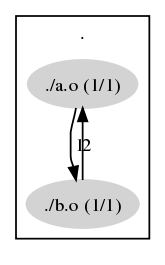
\includegraphics[scale=.5]{dep.png}
		\end{center}
	\end{columns}
\end{frame}


%%%%%%%%%%%%%%%%%%%%%%%%%%%%%%%%%%%%%%%%%%%%%%%%%%%%%%%%%%%%%%%%%%%%%%%%%%%%%%
%%%%%%%%%%%%%%%%%%%%%%%%%%%%%%%%%%%%%%%%%%%%%%%%%%%%%%%%%%%%%%%%%%%%%%%%%%%%%%
%%%%%%%%%%%%%%%%%%%%%%%%%%%%%%%%%%%%%%%%%%%%%%%%%%%%%%%%%%%%%%%%%%%%%%%%%%%%%%
\section{More...}
\begin{frame}[t]
	\frametitle{Fix the strange dependencies}
	\begin{itemize}
		\item<+-|alert@+> DIP (dependency inversion principle)
		\begin{enumerate}
			\item<+-|alert@+> High-level modules should not depend on low-level modules. Both should depend on abstractions.
			\item<+-|alert@+> Abstractions should not depend upon details. Details should depend upon abstractions.
		\end{enumerate}
		\item<+-|alert@+> design patterns
	\end{itemize}
\end{frame}

\begin{frame}[plain]
	\frametitle{A small experiment...}
	\begin{columns}
	\column{.5\textwidth}
		\begin{center}
			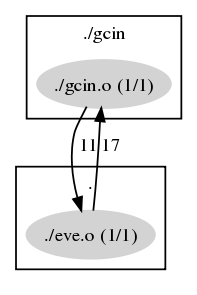
\includegraphics[scale=.4]{xim-demo-a.png}
		\end{center}

	\column{.5\textwidth}
		\begin{center}
			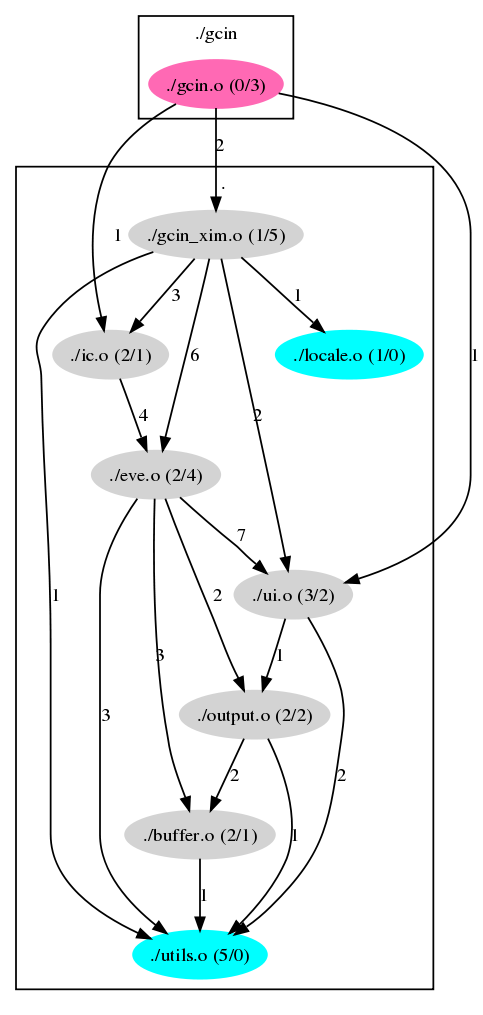
\includegraphics[scale=.2]{xim-demo-b.png}
		\end{center}
	\end{columns}
\end{frame}

\begin{frame}[t]
	\frametitle{Future Work}
	\begin{itemize}
		\item<+-|alert@+> package suggestion
		\item<+-|alert@+> dependency list generator for makefile
		\item<+-|alert@+> source code scanner
		\item<+-|alert@+> circular dependency detection
	\end{itemize}
\end{frame}

\begin{frame}
	\frametitle{Dependencies}
	\begin{center}
		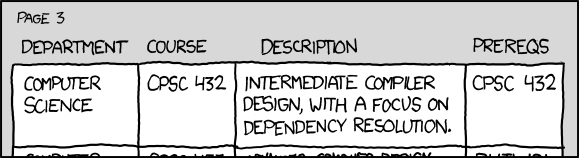
\includegraphics[scale=0.7]{xkcd754-dependencies.png}
		\begin{block}{Alt text}
		The prereqs for CPSC 357, the class on package management, are CPCS 432, CPSC 357, and glibc2.5 or later.
		\end{block}
		from \url{http://xkcd.com/754/}
	\end{center}
\end{frame}


%%%%%%%%%%%%%%%%%%%%%%%%%%%%%%%%%%%%%%%%%%%%%%%%%%%%%%%%%%%%%%%%%%%%%%%%%%%%%%
%%%%%%%%%%%%%%%%%%%%%%%%%%%%%%%%%%%%%%%%%%%%%%%%%%%%%%%%%%%%%%%%%%%%%%%%%%%%%%
%%%%%%%%%%%%%%%%%%%%%%%%%%%%%%%%%%%%%%%%%%%%%%%%%%%%%%%%%%%%%%%%%%%%%%%%%%%%%%
\section*{}
\begin{frame}[t]
	\frametitle{References}
	\begin{itemize}
		\item \href{http://networkx.lanl.gov/}{NetworkX}
		\item \href{http://www.graphviz.org/}{Graphviz}
		\item \href{http://www.doxygen.org/}{Doxygen}
		\item \href{http://www.catb.org/~esr/deheaderv/}{deheader}
%		\item \href{http://www-sop.inria.fr/mimosa/Olivier.Tardieu/software.html}{GDA Toolkit}
		\item \href{http://www.objectmentor.com/resources/articles/dip.pdf}{Dependency inversion principle}
	\end{itemize}
\end{frame}





\alertframe{\textit{Thank you!}}
\alertframe{\textit{Q \& A}}

%\begin{frame}<presentation>
%  \frametitle{Thanks}
%  \begin{center}
%  \textit{\huge Thanks for your attention!}~~~\textit{\large Q \& A}
%  \end{center}
%\end{frame}


\end{CJK}
\end{document}


